\newChapter{Implementation}{chap:dsl_implementation}

\section{Introduction}
\label{sec:implementation_intro}

In chapter~\ref{sec:implementation_of_a_dsl} we have introduced the
implementation of \gls{DSL} using the Scala programming language and why Scala
is a great choice for \gls{DSL} development.

This chapter deal with the implementation of the \gls{APDL} \gls{DSL} compiler
by showing and explaining the different part of the compilation process. We will
se the lexical and semantic analysis, the construction of the \gls{AST} and
finally the code generation.

Some specific part of the implementation are more complex so additional
information are given.

\section{Compilation Process}
\label{sec:compilation_process}

The whole \gls{APDL} compilation process is illustrated in figure
\ref{fig:apdl_compilation_process}. The compilation process is separated into
fours phases. Each phase receives an input and returns an output to the next
phases, except for the first and last ones. The four phases are :
\begin{itemize}
\item The lexical analyser receives the APDL source code and returns a first \gls{AST}.
\item The semantic analyser receive the \gls{AST} form the lexical analyser and
  return a symbol table and a second \gls{AST}, refined and more complete.
\item The code generator receive the symbol table and an \gls{AST} and generate
  the corresponding code in a file.
\item Code formatting, reformat the code inside the generated files.
\end{itemize}

The code formatting phase is not very important, it just provides a way to the
user to inspect the generated code and possibly find issues or errors.

\begin{figure}[!htbp]
  \centering
  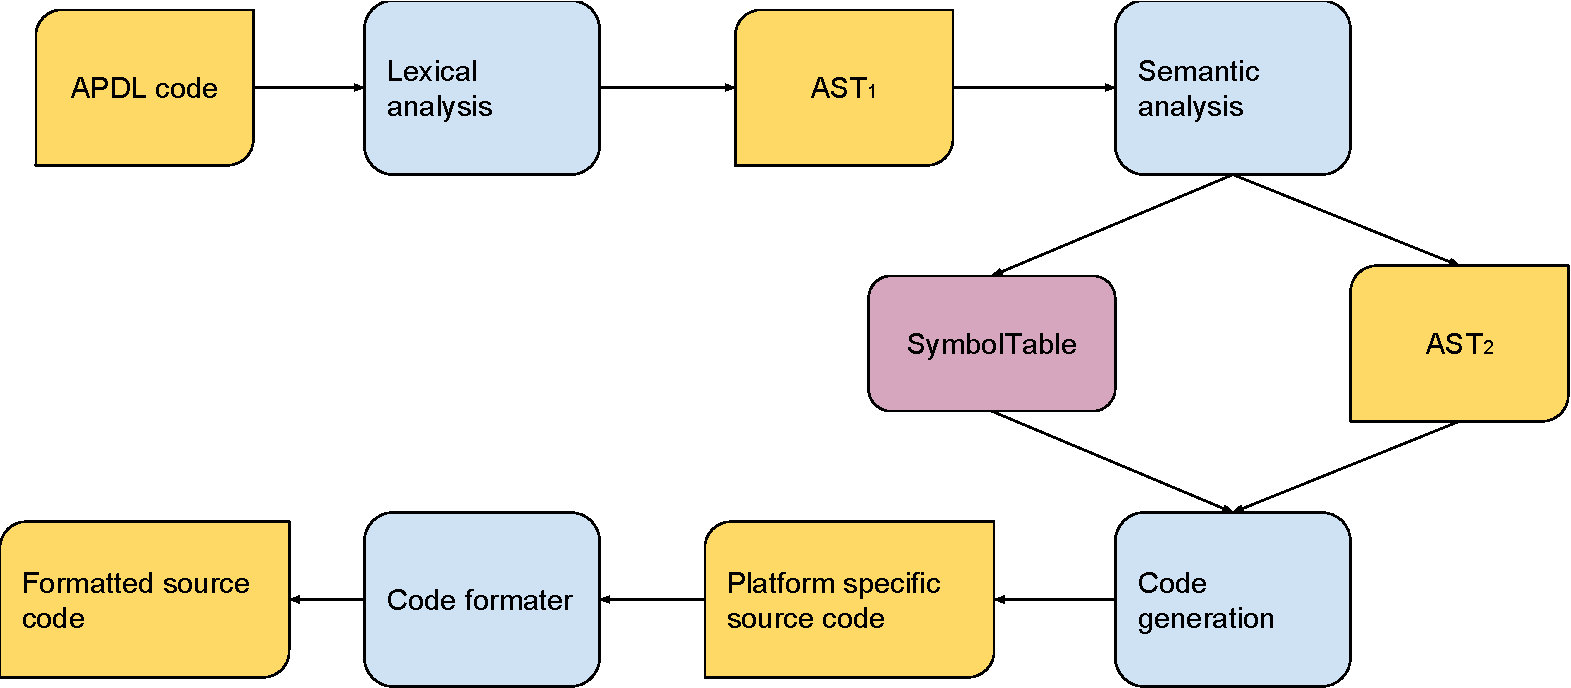
\includegraphics[width=0.9\textwidth]{img/compilation_process}
  \caption[APDL compilation process]{The APDL compilation process, the source
    code is parsed into a first \gls{AST} before transforming into a second one
    and a symbol table by the semantic analyser. Then, the code generator uses
    the \gls{AST} and the symbol table to generate a raw platform specific
    source code. Finally, a code formatter like Astyle\cite{TalDavidson}, ends the
    process in order to conveniently read the generated code.}
  \label{fig:apdl_compilation_process}
\end{figure}

\section{Lexical Analysis}
\label{sec:lexical_analysis}

The lexical analysis implementation has been achieved using the Scala
parser-combinator library\cite{Odersky:2016:PSU:2988396}. As explained
in~\ref{sec:multiple_dsl}, we have fragmented \gls{APDL} into multiple
\gls{DSL}. That means we have to parse the \gls{TF} and the main
languages.

So we have two parsers for our \gls{DSL}, a first one called
``TransformDSLParser'' and the second one called ``MainParser''. In fact, the
``MainParser'' has been separated into two more parsers, one for the user
definition and the second for the rest. But they could be seen as one.

The syntax of the \gls{TF} language is shown in listing \ref{lst:ebnf_tf}. The
syntax is close to some popular programming languages like Java, C or Scala. We
could note the absence of an ``end-of-statement'' symbol by opposition to C-like
languages.

\begin{listing}[!htbp]
  \centering
\begin{ebnfcode}
/* Types */
returnType ::= "void" | tfType
tfType ::= arrayType | primitiveType
arrayType ::= "[" "]" tfType
primitiveType ::= "bool" | numericType
numericType ::= integralType | floatingPointType
integralType ::= "int" | "long" | "char" | "short" | "byte"
floatingPointType ::= "float" | "double"

/* Expressions */
constantExpr ::= logicalOrExpr
logicalOrExpr ::= logicalOrExpr "||" logicalAndExpr | logicalAndExpr
logicalAndExpr ::= logicalAndExpr "&&" logicalEqExpr | logicalEqExpr
logicalEqExpr ::= logicalEqExpr "==" logicalRelationalExpr | logicalEqExpr "!=" logicalRelationalExpr | logicalRelationalExpr
logicalRelationalExpr ::= logicalRelationalExpr ">" additiveExpr | logicalRelationalExpr "<" additiveExpr | logicalRelationalExpr ">=" additiveExpr | logicalRelationalExpr "<=" additiveExpr | additiveExpr
additiveExpr ::= additiveExpr "+" multiplicativeExpr | additiveExpr "-" multiplicativeExpr | multiplicativeExpr
multiplicativeExpr ::= multiplicativeExpr "*" castExpr | multiplicativeExpr "/" castExpr | castExpr
castExpr ::= "(" primitiveType ")" castExpr | notExpr
notExpr ::= "!" notExpr | postfixExpr
postfixExpr ::= functionCall | arrayAccess | primaryExpr
functionCall ::= identifier "(" functionArgs ")"
arrayAccess ::= identifier ("[" constantExpr "]")+
primaryExpr ::= atom | symbol | literal | "(" constantExpr ")"
functionArgs ::= (constantExpr ("," constantExpr)*)?
atom ::= "true" | "false"
symbol ::= identifier
literal ::= [+-]?([0-9]+([.][0-9]*)?|[.][0-9]+)(E[0-9]+)?
identifier ::= [a-zA-Z_][a-zA-Z0-9_]*
assignExpr ::= postfixExpr "=" assignExpr | logicalOrExpr

/* Statement */
statement ::= block | selectionStatement | loops | jump | declaration | exprStatement
block ::= "{" (statement)* ")"
selectionStatement ::= ifThenElse | ifThen
loops ::= while | doWhile
jump ::= "break" | "continue" | "return" constantExpr
declaration ::= newVar | newArray | newVal | functionDeclaration
exprStatement ::= constantExpr
ifThenElse ::= "if" "(" constantExpr ")" statement "else" statement
ifThen ::= "if" "(" constantExpr ")" statement
while ::= "while" "(" constantExpr ")" statement
doWhile ::= "do" statement "while" "(" constantExpr ")"
newVar ::= "var" identifier ":" tfType "=" constantExpr | "var" identifier ":" tfType
newArray ::= "var" identifier ":" arrayType "=" arrayInit | "var" identifier ":" arrayType
newVal ::= "val" identifier ":" tfType "=" constantExpr
functionDeclaration ::= "def" functionHeader functionBody
arrayInit ::= "[" literal "]" | "{" constantExpr ("," constantExpr)* "}"
functionHeader ::= identifier "(" (arg ("," arg)*)? ")" "->" returnType
functionBody ::= block
arg ::= identifier ":" tfType
\end{ebnfcode}
  \caption[EBNF syntax of the Transform APDL Language]{EBNF syntax of the
Transform APDL Language. The syntax is similar to C and Java, except that there
is no need to specify an ``end-of-statement''.}
  \label{lst:ebnf_tf}
\end{listing}

The syntax for defining new components, inputs or transformations is available
in listing~\ref{lst:ebnf_defines}, the one for the main \gls{DSL} in
listing~\ref{lst:ebnf_all}.

\begin{listing}[!htbp]
  \centering
  \begin{ebnfcode}
defines ::= (define)*
define ::= "@define" (defineComponent | defineInput | defineTransform)
defineComponent ::= "component" identifier parameters "{" defineComponentBody "}"
defineInput ::= "input" identifier parameters "{" gens "}"
defineTransform ::= "transform" functionDeclaration
parameters ::= (parameter)*
parameter ::= identifier ":" type
defineComponentBody ::= inputs output gens
gens ::= (gen)*
gen ::= "@gen" identifier "{" genBody "}"
inputs ::= "@in" parameters
output ::= "@out" type
type ::= "str" | "id" | stdType
stdType ::= "int" | "long" | "char" | "short" | "byte" | "float" | "double"
genBody ::= global setup loop expr genType
global ::= "global" "=" '"' literalString '"'
setup ::= "setup" "=" '"' literalString '"'
loop ::= "loop" "=" '"' literalString '"'
expr ::= "expr" "=" '"' literalString '"'
genType ::= "type" "=" stdType
literalString ::= (.|[^\"])*
  \end{ebnfcode}
  \caption[EBNF syntax for APDL's new definition]{EBNF syntax for defining new
components, inputs and transformations. The EBNF nodes that aren't in this
syntax are in the syntax from listing \ref{lst:ebnf_tf}.}
  \label{lst:ebnf_defines}
\end{listing}

\begin{listing}[!htbp]
  \centering
  \begin{ebnfcode}
program ::= (projectName | apdlDevice | define)+
projectName ::= "project_name" "=" '"' literalString '"'
apdlDevice ::= "@device" identifier "{" (keyValue | apdlInput | apdlSerial)+ "}"
apdlInput ::= "@input" identifier identifier apdlParameters
apdlSerial ::= "@serial" identfier apdlSampling
apdlParameters ::= (apdlParameter)*
apdlParameter ::= "[^ \t\f\n\r{}@]+"
apdlSampling ::= apdlSamplingUpdate | apdlSamplingTimer
apdlSamplingUpdate ::= "update"
apdlSamplingTimer ::= "each" '[0-9]+' timeUnit
timeUnit ::= "ns" | "ms" | "s" | "m" | "h" | "d"
  \end{ebnfcode}
  \caption[EBNF syntax for the \gls{APDL} \gls{DSL}]{The full EBNF syntax for
the \gls{APDL} \gls{DSL}. Any language accepted by this grammar is a valid,
syntactically speaking, \gls{APDL} program. The EBNF nodes that aren't in this
syntax are in the syntax from listing \ref{lst:ebnf_defines}.}
  \label{lst:ebnf_all}
\end{listing}

The implementation of the parsers has been achieved by using a specific parser
from the Scala parser-combinator library. Precisely, we have used a parser
technique called the packrat parser\cite{Ford2006}. Parsing grammar with
packrat parser is guaranteed to operate in a linear time through the use of
memoization\cite{Ford2006}. Packrat parser also allows the usage of left
recursion, which is significant with the type of grammar we used for defining the
syntax of our \gls{APDL}.

As an example for the packrat algorithm, we would take the grammar of the
``additiveExpr'' :

\begin{inlineebnf}
additiveExpr ::= additiveExpr "+" multiplicativeExpr
             | additiveExpr "-" multiplicativeExpr
             | multiplicativeExpr
\end{inlineebnf}

If we use a standard algorithm in order to implement this grammar, we would
have something like

\begin{inlinescala}
def tfAdditiveExpr: Parser[Expr] = {
  tfAdditiveExpr ~ ("+" ~> tfMultiplicativeExpr) ^^ {
    case (l ~ r) => Add(l, r)
  } |
  tfAdditiveExpr ~ ("-" ~> tfMultiplicativeExpr) ^^ {
    case (l ~ r) => Sub(l, r)
  } |
  tfMultiplicativeExpr
}
\end{inlinescala}

The problem with this implementation is the infinite recursive call which
happens, because the first rule of the token is the token itself.
Using packrat parser solves this problem by enabling the left
recursion as well as using memoization through lazy evaluation :

\begin{inlinescala}
lazy val tfAdditiveExpr: PackratParser[Expr] = {
  tfAdditiveExpr ~ ("+" ~> tfMultiplicativeExpr) ^^ {
    case (l ~ r) => Add(l, r)
  } |
  tfAdditiveExpr ~ ("-" ~> tfMultiplicativeExpr) ^^ {
    case (l ~ r) => Sub(l, r)
  } |
  tfMultiplicativeExpr
}
\end{inlinescala}

This time, it's a lazy value so we don't have an immediate infinite recursion. So
the packrat algorithm can operate and enables the left recursion.

During the lexical analysis, the parsers are producing the \gls{AST} of the
program. In Scala, the \gls{AST} is designed and built by using case classes and
sealed traits. We are not going to present the whole implementation of the
\gls{AST}, all the code is available in appendix
\ref{app:apdl_ast_implementation}. We will just present the implementation for
the expression of the \gls{TF} Language, the code is shown in listing
\ref{lst:ast_implementation}.

\begin{listing}[!htbp]
  \centering
  \begin{scalacode}
sealed trait ApdlAst

sealed trait Expr extends ApdlAst
// Arithmetic expression
case class Add(left: Expr, right: Expr) extends Expr
case class Mul(left: Expr, right: Expr) extends Expr
case class Sub(left: Expr, right: Expr) extends Expr
case class Div(left: Expr, right: Expr) extends Expr
case class Cast(tfTyp: TfPrimitivesTyp, expr: Expr) extends Expr
case class Literal(value: String) extends Expr
case class Symbol(name: String) extends Expr
case class FunctionCall(funcName: String, args: List[Expr]) extends Expr
case class ArrayAccess(array: Expr, field: Expr) extends Expr
case class VarAssignement(target: Expr, value: Expr) extends Expr

// Boolean expression
case class True() extends Expr
case class False() extends Expr
case class Or(left: Expr, right: Expr) extends Expr
case class And(left: Expr, right: Expr) extends Expr
case class Not(expr: Expr) extends Expr
case class Greater(left: Expr, right: Expr) extends Expr
case class Smaller(left: Expr, right: Expr) extends Expr
case class GreaterEquals(left: Expr, right: Expr) extends Expr
case class SmallerEquals(left: Expr, right: Expr) extends Expr
case class Equals(left: Expr, right: Expr) extends Expr
case class NotEquals(left: Expr, right: Expr) extends Expr
  \end{scalacode}
  \caption[\gls{APDL} \gls{AST} implementation in Scala]{Implementation of the
\gls{APDL} abstract syntax tree using case classes and sealed traits. The usage
of inheritance is very powerful.}
  \label{lst:ast_implementation}
\end{listing}

The full set of syntactical diagrams is available in appendix
\ref{app:apdl_ebnf_diagramm}. We also need to mention that the parser is not
performing any verification of the input's semantics, that's the semantics
analyser role.

\section{Semantic Analysis}
\label{sec:semantic_analysis}

The semantic analyser role is to construct the symbol table of the \gls{APDL}
compiler. The symbol table is just a map where the key is the identifier of a
definition or a variable inside a device, and the value is the \gls{AST} of the
corresponding definition or user implementation.

The implementation of the symbol table is available in
listing~\ref{lst:symbol_table_implementation}. The semantic analyser builds the
table, especially the input, by recursively walking through the \gls{AST} and
generating the corresponding values for the symbol table.

\begin{listing}[!htbp]
  \centering
\begin{scalacode}
sealed trait SymbolTableElement

case class Component(identifier: String,
                     outputType: ApdlType,
                     parameters: List[Parameter]) extends SymbolTableElement
case class Transform(functionDecl: FunctionDecl) extends SymbolTableElement

sealed trait Input extends SymbolTableElement {
  def getDefinition: ApdlDefine = this match {
    case InputDefault(_, definition, _, _) => definition
    case InputTransformed(_, definition, _) => definition
    case InputComponented(_, definition, _) => definition
  }
}

case class InputDefault(identifier: String,
                        definition: ApdlDefineInput,
                        args: List[String],
                        expr: String) extends Input
case class InputTransformed(identifier: String,
                            definition: ApdlDefineTransform,
                            input: Input) extends Input
case class InputComponented(identifier: String,
                            definition: ApdlDefineComponent,
                            inputs: List[Input]) extends Input
\end{scalacode}
  \caption[Scala's implementation of the symbol table accepted values]{Implementation of the
symbol table accepted values using sealed trait and case classes. Basically,
it's just a map with a few methods and a typed value for
correctness.} \label{lst:symbol_table_implementation}
\end{listing}

The \gls{AST} generated by the parser is very simple and is just a translation of
the program into traits and case classes. If we take the input

\begin{inlineapdl}
@device arduino1 {
    id = uno
    framework = arduino
    @input rawTemp analogInput 1
    @input temp tf rawTemp
    @input temp2 tf temp
    @serial temp2 update
}
\end{inlineapdl}

we saw that the $temp2$ value is built with the $temp$ value, which is built
with the $rawTemp$ value. So we could define a graph $G$ of inputs : $G =
rawRemp \rightarrow temp \rightarrow temp2$ , where $\rightarrow$ means ``is
input of''.

The previous graph is linear and could be just seen as a list. When component
comes into play, we could have multiple inputs for a same node of the graph and
we obtain a tree. Note that defining components with multiple outputs is not yet
permitted by \gls{APDL} but is planned for the future.

In order to construct the whole recursive inclusion of inputs, we need, at first,
to generate the inputs located in the leaves of the tree. Then, we generate
the nodes that are already known inputs and we repeat that
until we got the full inputs set done. The algorithm is described in
Algorithm\ref{alg:recurisive_inclusion_construct}.

\begin{algorithm}[!htbp]
  \centering
  \begin{algorithmic}[5]
    \State List of non-leaf inputs : $is$
    \State Symbol table : $s$
    \Repeat
    \State $(generableInput,nonGenerableInputs) \gets is.partition(isGenerable)$
    \For{$i \in is$}
    \If{$i : Transform$}
    \State $sourceInput \gets s.get(\text{first argument of $i$})$
    \State $key \gets \text{Identifier of $i$}$
    \State $value \gets Transform(\text{AST of the function declaration},sourceInput)$
    \State $s.put(key,value)$
    \EndIf
    \If{$i : Component$}
    \State $args \gets \text{Input identifier of $i$}$
    \State $sourceInputs \gets s.get(args)$
    \State $key \gets \text{Identifier of $i$}$
    \State $value \gets ComponentedInput(key,\text{Definition AST of $i$},sourceInputs)$
    \State $s.put(key,value)$
    \EndIf
    \EndFor
    \Until{$is$ is empty}
  \end{algorithmic}
  \caption[Recursive inclusion construction]{Recursive inclusion
    construction algorithms. The Scala implementation is available in appendix \ref{app:algo_recursive_construct}.}
  \label{alg:recurisive_inclusion_construct}
\end{algorithm}

A Scala implementation of the algorithm~\ref{alg:recurisive_inclusion_construct}
is available in appendix~\ref{app:algo_recursive_construct}. The implementation
is recursive and also processes some verification on the types of the data and on the
presence of the identifier in the symbol table.

We also need to note that there is mostly no type system, type verification or
semantic verification of the code at the compile time. It requires a lot of work
to build a strong verification system, and the time allowed for this work is too
short. The user needs to be extremely worried about his code, and the
errors that he encounters could have been found before the runtime.
Implementing a good type system and more verification is planned for the future.

\section{Code Generation}
\label{sec:code_generation}

There are multiple parts in the code generation process :
\begin{itemize}
\item Generating the project folders and the script for launching the application.
\item Generating the PlatformIO project for a device.
\item Generating the code for a specific device, including inputs, serial
  sends, transformation functions and components.
\end{itemize}

The project and device generation is quite simple and does not require a lot of
explanations. Basically, it's just a set of new folders and PlatformIO ``.ini''
files for each device. A bash script is also produced in order to launch the
whole application.

The code generation is a lot more interesting. Firstly, we have seen in
chapter~\ref{sec:framework_for_embeded_dev} ,that a lot of various
frameworks are available. Each framework has its vision on how to implement a device. For
example, Arduino offers two methods, $loop$ and $setup$, that offers the eponym
functionality to the user. Mbed does not have this, and we have to simulate them.

For this purpose, we have developed an abstraction for the code generation. The
code to generate is the same for both the Mbed and Arduino frameworks, but the
location to generate it differs from one to the other. Both listings
\ref{lst:pw_arduino} and \ref{lst:pw_mbed} for Arduino, respectively Mbed,
show both implementations.

\begin{listing}[!htbp]
  \centering
\begin{scalacode}
override def close(): Unit = {
    pw.append {
      s"""
         |#include <stdbool.h>
         |${if (generateTimer) s"""#include "Timer.h""""}
         |
         |${if (generateTimer) s"Timer t;"}
         |
         |// Global definition
         |${global.toString}
         |
         |// Function definition
         |${function.toString}
         |
         |void loop() {
         |  ${if (generateTimer) s"t.update();"}
         |  ${loop.toString}
         |}
         |
         |void setup() {
         |  ${if (generateSerial) s"Serial.begin(9600);"}
         |  ${setup.toString}
         |}
         |
       """.stripMargin
    }
    pw.flush()
    pw.close()
    formatSource()
  }
}
\end{scalacode}
  \caption[Implementation of the code generation location for
Arduino]{Implementation of the Mbed code generation location. The code is
generated by using Stringwriter. The compiler accumulates the generated code in
buffer until the end of the compilation. At the end, the compiler interpolates
the string with the contents of his buffers.}
\label{lst:pw_arduino}
\end{listing}

\begin{listing}[!htbp]
  \centering
\begin{scalacode}
override def close(): Unit = {
    pw.append {
      s"""
         |#include <stdbool.h>
         |#include <mbed.h>
         |
         |${if (generateTimer) s"Ticker ticker;"}
         |
         |${if (generateSerial) s"Serial pc(USBTX, USBRX);"}
         |
         |// Global definition
         |${global.toString}
         |
         |// Function definition
         |${function.toString}
         |
         |int main(void) {
         |  ${if (generateSerial) s"pc.baud(4800);"}
         |  // Setup
         |  ${setup.toString}
         |
         |  // Loop
         |  while(1) {
         |    ${loop.toString}
         |  }
         |  return 0;
         |}
         |
       """.stripMargin
    }
    pw.flush()
    pw.close()
    formatSource()
  }
\end{scalacode}
  \caption[Implementation of the code generation location for
Mbed]{Implementation of the Mbed code generation location. The code is generated
by using Stringwriter. The compiler accumulate the generated code in buffer
until the end of the compilation. At the end, the compiler interpolate the
string with the contents of his buffers.}
\label{lst:pw_mbed}
\end{listing}

Another improvement we can do about the code generation is the management of the
frameworks specific objects. For example the Timer/Ticker class in Mbed and
Arduino. Arduino allow only ten callback per Timer object and for the moment
there is no verification about it. The general improvement is about creating
classes that manage the behaviour of the framework specific object we need and
make an abstraction for those.

The code generation for the \gls{TF} language is also simple to implements. The
use of sealed traits and case classes allow us to use recursive methods in order
to generate an appropriate C source code. As an example,
listing~\ref{lst:expr_code_generation} showed the implementation of the code
generation only for the expressions from the \gls{TF} language. The code is
recursively generated by using pattern matching on the \gls{AST} tokens.

\begin{listing}[!htbp]
  \centering
\begin{scalacode}
// ...
def apply(apdlAst: ApdlAst): String = apdlAst match {
  case e: Expr => e match {
    case Add(left, right) => s"(${apply(left)} + ${apply(right)})"
    case Mul(left, right) => s"(${apply(left)} * ${apply(right)})"
    case Sub(left, right) => s"(${apply(left)} - ${apply(right)})"
    case Div(left, right) => s"(${apply(left)} / ${apply(right)})"
    // ...
  }
case t : TfRetType => t match {...}
// ...
\end{scalacode}
  \caption[Implementation of the code generation for
expressions]{Implementation, in Scala, of the code generation for \gls{TF}
language expressions. Case classes allow the heavy use of pattern matching and
recursive call to compute the whole \gls{AST}.}
  \label{lst:expr_code_generation}
\end{listing}

The \gls{APDL} compiler do not really act as a compiler for the moment. It
acts like a code translator from \gls{APDL} to C/C++ with some adjustment in
function of the chosen framework for a device.

The last point to mention is about the scope identifier collision. If a user
defines a new component like the following.
\begin{inlineapdl}
@define component loopCounter {
    @in
    @out int
    @gen arduino {
        global = "int a;"
        setup = "a = 0"
        loop = "a = a + 1;"
        expr = "a"
  }
}
\end{inlineapdl}
The user absolutely don't know if the identifier $a$ or $loopCounter$ is already
defined by another definition or by \gls{APDL} itself. The lack of such a
verification system is not yet implemented in \gls{APDL} and, as well as other
features, is planned for the future.

\section{Summary}
\label{sec:implementation_summary}

This chapter has presented the actual implementation of the \gls{APDL} compiler.
The main idea to remind is the compilation process illustrated in
figure~\ref{fig:apdl_compilation_process}. The raw source code is firstly parsing
into a simple \gls{AST} before generating into a symbol table. Finally, the code
generator uses the symbol table and the remaining \gls{AST} for the code
generation.

We also note that the compiler is by far not finish and a lot of major
features and improvements has to be done before having a real product. Some of
those features are :

\begin{itemize}
\item Type verification during the compilation time.
\item A better type system in general.
\item Verification about the scope collision in new definition.
\item Some modules which simplify the management of framework specific entities. 
\end{itemize}

This is a non-exhaustive list and \gls{APDL} probably owns several more issues
and possible improvements.

Finally, we present the skeleton process for the code generation by showing a
small code(\ref{lst:expr_code_generation}) that generate the C code for the
expression.

%%% Local Variables:
%%% mode: latex
%%% TeX-master: "../thesis"
%%% End: